\documentclass[UTF8, a4paper, linespread=1.5]{article}

\usepackage{tcolorbox, listings, algorithm, minted, algpseudocode}
\usepackage{geometry, savesym, amsmath, enumerate, indentfirst, color, amsthm, bm, extarrows, ulem}
\usepackage{amssymb}
\usepackage{nameref, hyperref}
 \geometry{top=3cm, bottom=3cm, left=1.5cm, right=1.5cm}

\usepackage{enumitem}
\setenumerate[1]{itemsep=0pt,partopsep=0pt,parsep=\parskip,topsep=5pt}
\setitemize[1]{itemsep=0pt,partopsep=0pt,parsep=\parskip,topsep=5pt}

\renewcommand\contentsname{Contents}

\tcbuselibrary{skins, breakable, theorems}

% \setlength{\leftskip}{10pt}
\setlength{\parindent}{10pt}
% \setlength{\parskip}{2em}
\renewcommand{\baselinestretch}{1.3}

\newcounter{RomanNumber}
\newcommand{\mrm}[1]{(\setcounter{RomanNumber}{#1}\Roman{RomanNumber})}

\newtcbtheorem{thm}{}
  {enhanced, theorem name and number, code={\edef\@currentlabelname{#2}}, 
  frame code={
        % \path[thick, draw] (frame.north west) -| (frame.north east) -| (frame.south east) -| (frame.south west) -| (frame.north west);
        \path[thick, draw] (frame.north west)  +(.5\baselineskip,0) -| +(0,-.5\baselineskip);
        % \path[thick, draw] (frame.north east) +(-.5\baselineskip,0) -| +(0,-.5\baselineskip);
        % \path[thick, draw] (frame.south west) +(.5\baselineskip,0) -| +(0,.5\baselineskip);
        \path[thick, draw] (frame.south east) +(-.5\baselineskip,0) -| +(0,.5\baselineskip);
    },
    left=1mm, right=1mm, top=1mm, bottom=1mm,
    colback=black!5,
    colframe=red!75!black,
    colbacktitle=black!0,
    coltitle=black!100,
    fonttitle=\bfseries}{thm}


\usepackage{environ}
\RenewEnviron{math}{%
\begin{align*}
\BODY
\end{align*}
}

\title{CS217 -- Algorithm Design and Analysis \\ Homework 5}
\date{\today}
\author{Not Strong Enough}



\begin{document}
\maketitle

\begin{thm}{}{}
    Given an array $A$ of $n$ items (numbers), we can find the maximum with $n - 1$ comparisons (this is simple). Show that this is optimal: that is, any algorithm that does $n - 2$ or fewer comparisons will fail to find the maximum on some inputs.
\end{thm}

\begin{proof}
    No matter how we make the comparisons and finally get the maximum, the process of finding the maximum forms a "comparision tree". Now we explain how the "comparison tree" is formed:
    
    \begin{enumerate}
        \item At the beginning, each item of $A$ is regarded as a node, and all nodes are separated. Each node has a value such as $A[0], A[1], \ldots, A[n - 1]$.
        \item Each time we pick two nodes $a$ and $b$ such that both $a$ and $b$ have \textbf{no parent} in the tree.
        \item Then we make a comparison between the values of $a$ and $b$, and get the larger one. 
        \item We add a new node as the parent of both $a$ and $b$. The value of the new node is set to $\max\{a, b\}$.
        \item Repeat step 2 to step 4. Stop when there is only one node which has no parent, i.e., all nodes constitute a tree. Finally the value of the root is the maximum, which is what we want.
    \end{enumerate}
    
    From the process, we know that the leaves of the tree are the very $n$ origin nodes. And it is clear that every internal node, i.e., node that is not a leaf, has exactly two children, since the internal node is added after comparing its two children.
    
    Now the number of comparisons equals the number of internal nodes in the "comparison tree". At the beginning, the number of nodes which have no parent is $n$, and there is no internal node. Everytime we make a comparison, we add a new node as the parent of two nodes which have no parent. So the number of nodes which have no parent decreases $2 - 1 = 1$, and the number of internal nodes increases $1$. Finally there is only one node which is the root. So step 2 to step 4 repeats $n - 1$ times, and number of internal nodes equals $n - 1$.
    
    Therefor, at least $n - 1$ comparisons are needed. Otherwise we will get more than one tree in the end, and thus we cannot determine which value is the maximum.
    
    \paragraph{Another explanation}
    \label{anotherExplanation}
    For each number $x$ which is not the maximum, there must be at least one comparison between $x$ and a number larger than or equal to $x$. If not, we may also regard $x$ as the maximum since we don't ever find a number larger than or equal to it. Because there are $n - 1$ numbers which are not the maximum, finding the maximum needs at least $n - 1$ comparisons.
\end{proof}

\newpage

\begin{thm}{}{}
    Let $A$ be an array of size $n$, where $n$ is even. Describe how to find both the minimum and the maximum with at most $\frac{2}{3}n - 2$ comparisons. Make sure your solution is \textit{simple}, in describe it in a clear and succinct way!
\end{thm}

\begin{proof}[Solution]
    Since $n$ is even, we can divide $A$ into $n / 2$ pairs, and the elements of the $i$-th pair are $A[2i]$ and $A[2i + 1]$.
    
    At the beginning, compare $A[0]$ and $A[1]$. Let $maximum$ be the larger one and $minimum$ be the smaller one.
    
    For pair $i(i = 1, 2, \ldots, n - 1)$, compare $A[2i]$ and $A[2i + 1]$ at first. Then we compare the larger one with $maximum$. If the larger one is greater than $maximum$, let $maximum$ be the larger one. Similarly, we then compare the smaller one with $minimum$, and if the smaller one is less than $minimum$, let $minimum$ be the smaller one.
    
    In the end we get both the $maximum$ and the $minimum$ of $A$.
    
    Now we calculate the number of comparisons. For the $0$-th pair, we made only $1$ comparison. For other pairs, we made exactly $3$ comparisons. So the total number of comparisons is $1 + (\frac{n}{2} - 1) \cdot 3 = \frac{3n}{2} - 2$, which satisfy the requirement.
\end{proof}

Here is the pseudocode of the algorithm above.
\begin{algorithm}
    \caption{Find both the maximum and minimum of an array within $\frac{3n}{2} - 2$ comparisons.}
    \begin{algorithmic}
        \Ensure $n$ is even
        \Function{FindMaxAndMin}{$A$, $n$}
        
        \State $m \gets n / 2$
        \If{$A[0] > A[1]$}
            \State $maximum \gets A[0]$
            \State $minimum \gets A[1]$
        \Else
            \State $maximum \gets A[1]$
            \State $minimum \gets A[0]$
        \EndIf
        
        \For{$i \gets 1$ to $(n - 1)$}
            \If{$A[2i] > A[2i + 1]$}
                \State $maximum \gets \max\{maximum, A[2i]\}$
                \State $minimum \gets \min\{minimum, A[2i + 1]\}$
            \Else
                \State $maximum \gets \max\{maximum, A[2i + 1]\}$
                \State $minimum \gets \min\{minimum, A[2i]\}$
            \EndIf
        \EndFor
        \\\ \ \ \ \Return $maximum, minimum$
        \EndFunction
    \end{algorithmic}
\end{algorithm}

\newpage

\begin{thm}{}{}
    Given an array $A$ of size $n = 2^k$, find the second largest element with at most $n + \log_2(n)$ comparisons. Again, your solution should be \textit{simple}, and you should explain it in a clear and succinct way!
\end{thm}

\begin{proof}[Solution]
    Firstly we consider the following process of finding the maximum recursively.
    
    We divide the array into 2 parts with the same length. Then we find the maximum of both left and right part recursively. And finally we return the larger one between the two maximums of the left and right part. According to exercise 1, it takes $n - 1$ comparisons to find the maximum.
    
    Consider maximum of the whole array. During the process above, the maximum was compared to exactly $\log_2(n)$ element, since there are $\log_2(n) + 1$ levels in the "comparison tree" and in each level except the top one, the maximum was compared to another element.
    
    Among the $\log_2(n)$ elements which were compared to the maximum, there must be the second largest element of the whole array. Otherwise assume the second largest element is $x'$, and there is no direct comparison between the largest and the second largest element $x'$. Then either $x'$ is not the second largest at all if there exists some "indirect comparison" between $x'$ and the maximum, or according to the second explanation of exercise 1, we may also regard $x'$ as the maximum since we didn't even find an element which is larger than or equal to $x'$!
    
    So we just need to collect the $\log_2(n)$ elements which were compared to the maximum(this is not difficult because we can record down the elements compared to each element in each level of the "comparison tree"). Then we use $\log_2(n) - 1$ comparisons to find the maximum among the $\log_2(n)$ elements. What we get in the end is the second largest element of the whole array.
    
    Therefore, the total number of comparisons is $(n - 1) + (\log_2(n) - 1) = n + \log_2(n) - 2$, which is less than the required number $n + \log_2(n)$.
\end{proof}

We also offer a pseudocode of this algorithm.
\begin{algorithm}
    \caption{Find the second largest element with at most $n + \log_2(n)$ comparisons.}
    \begin{algorithmic}
        \Ensure $n = 2^k$
        \Function{FindMaximumIndex}{$A$, $left$, $right$}
            \If{$left + 1 = right$}
            
                \ \ \ \Return $left, [\ ]$
            \EndIf
            
            \State $mid \gets (left + right) / 2$
            \State $max_L, list_L \gets$ \Call{FindMaximumIndex}{$A$, $left$, $mid$}
            \State $max_R, list_R \gets$ \Call{FindMaximumIndex}{$A$, $mid$, $right$}
            
            \If{$A[max_L] > A[max_R]$}
                \State append $max_R$ to $list_L$
                
                \ \ \ \Return $max_L, list_L$
            \Else
                \State append $max_L$ to $list_R$
                
                \ \ \ \Return $max_R, list_R$
            \EndIf
        \EndFunction
        
        \\
        \Function{FindSecondLargestElement}{$A$, $n$}
            \State $max, list \gets$ \Call{FindMaximumIndex}{$A$, $0$, $n$}
            \State $k \gets \log_2(n)$
            \State $secondLargest \gets A[list[0]]$
            \For{$i \gets 1$ to $(k - 1)$}
                \If{$A[list[i]] > secondLargest$}
                    \State $secondLargest \gets A[list[i]]$
                \EndIf
            \EndFor
            \\\ \ \ \ \Return $secondLargest$
        \EndFunction
    \end{algorithmic}
\end{algorithm}

\newpage

\begin{thm}{}{}
    Explain how QuickSelect can be viewed as a “partial execution” of quicksort with the random pivot selection rule. Draw an example quicksort tree and show which part of this tree is visited by QuickSelect.
\end{thm}

\begin{figure}[htpb]
    \centering
    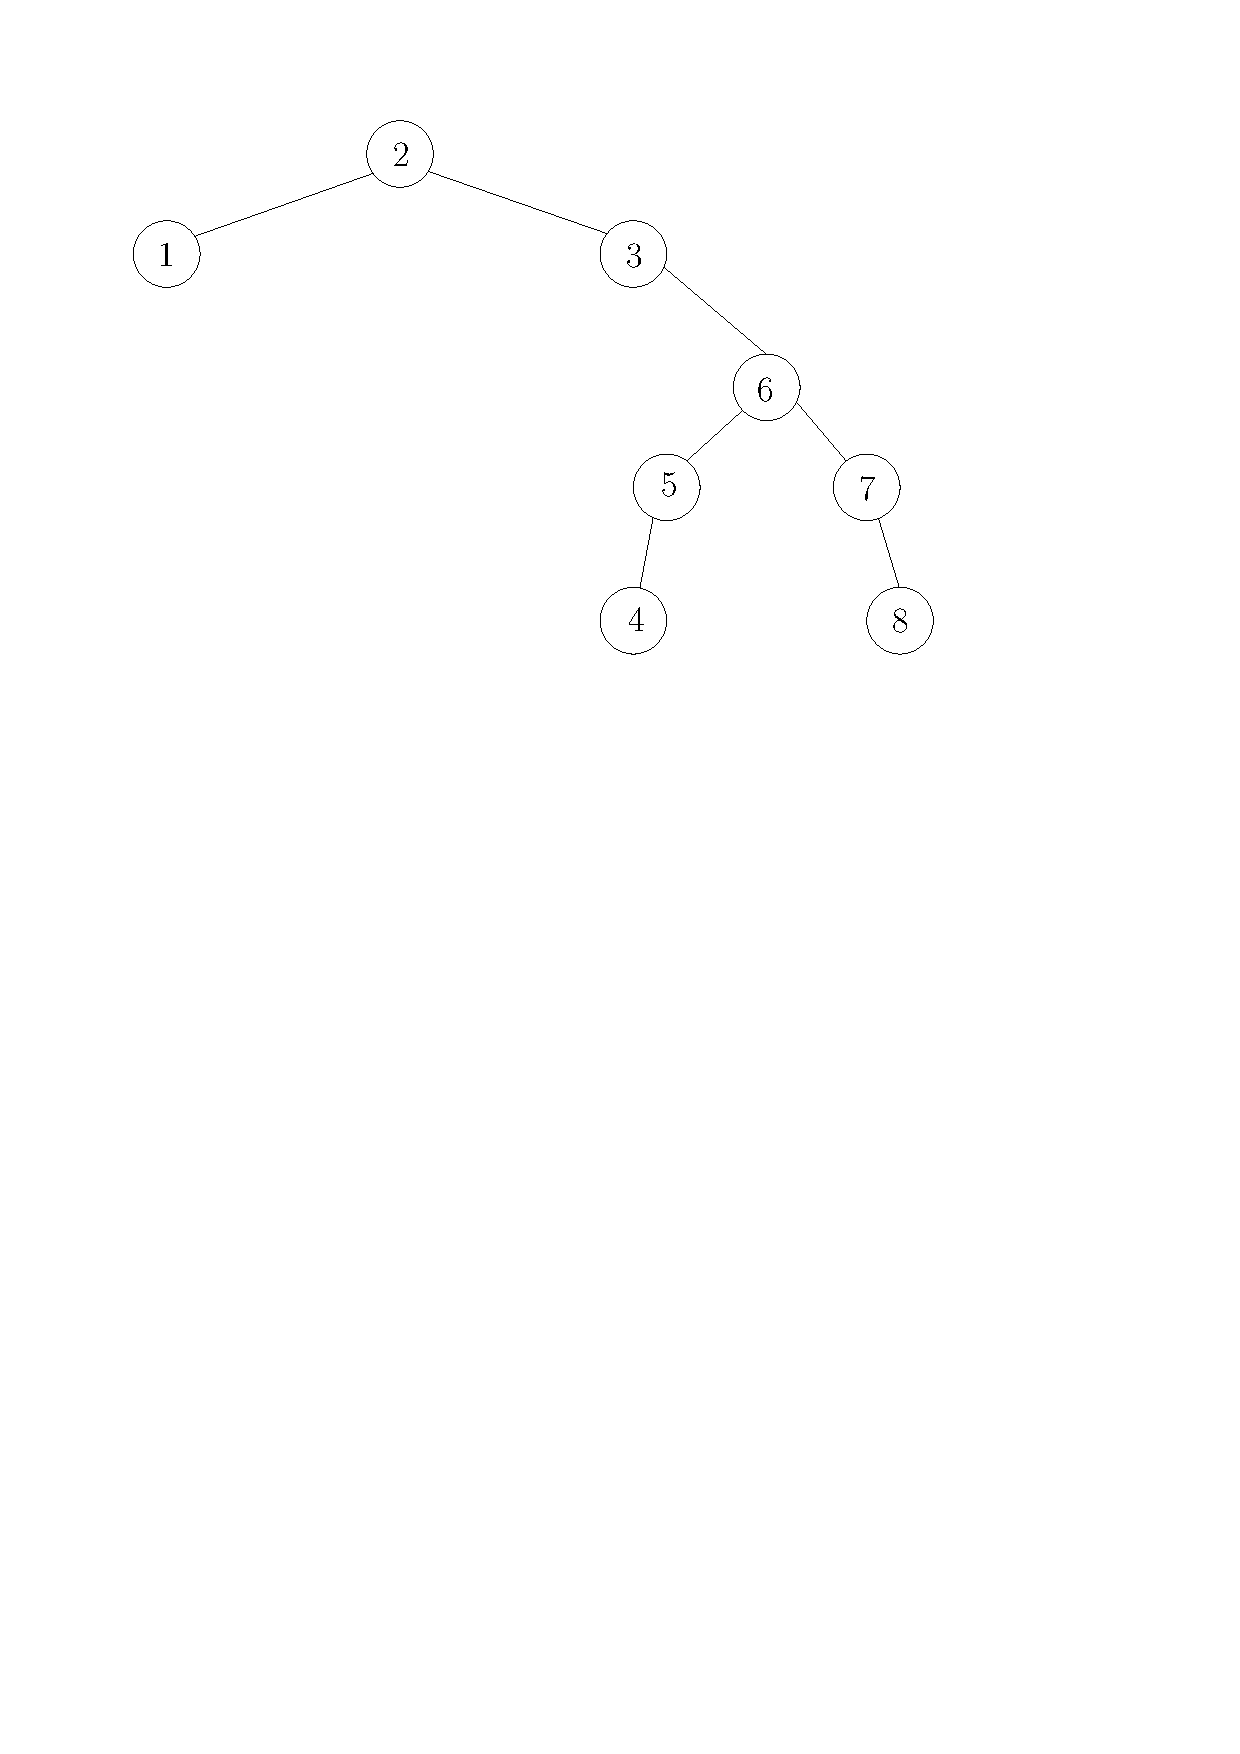
\includegraphics[width=0.6\textwidth]{qsort.pdf}
    \caption{quicksort tree of $[2,3,6,1,7,5,8,4]$}
\end{figure}
\begin{figure}[htpb]
    \centering
    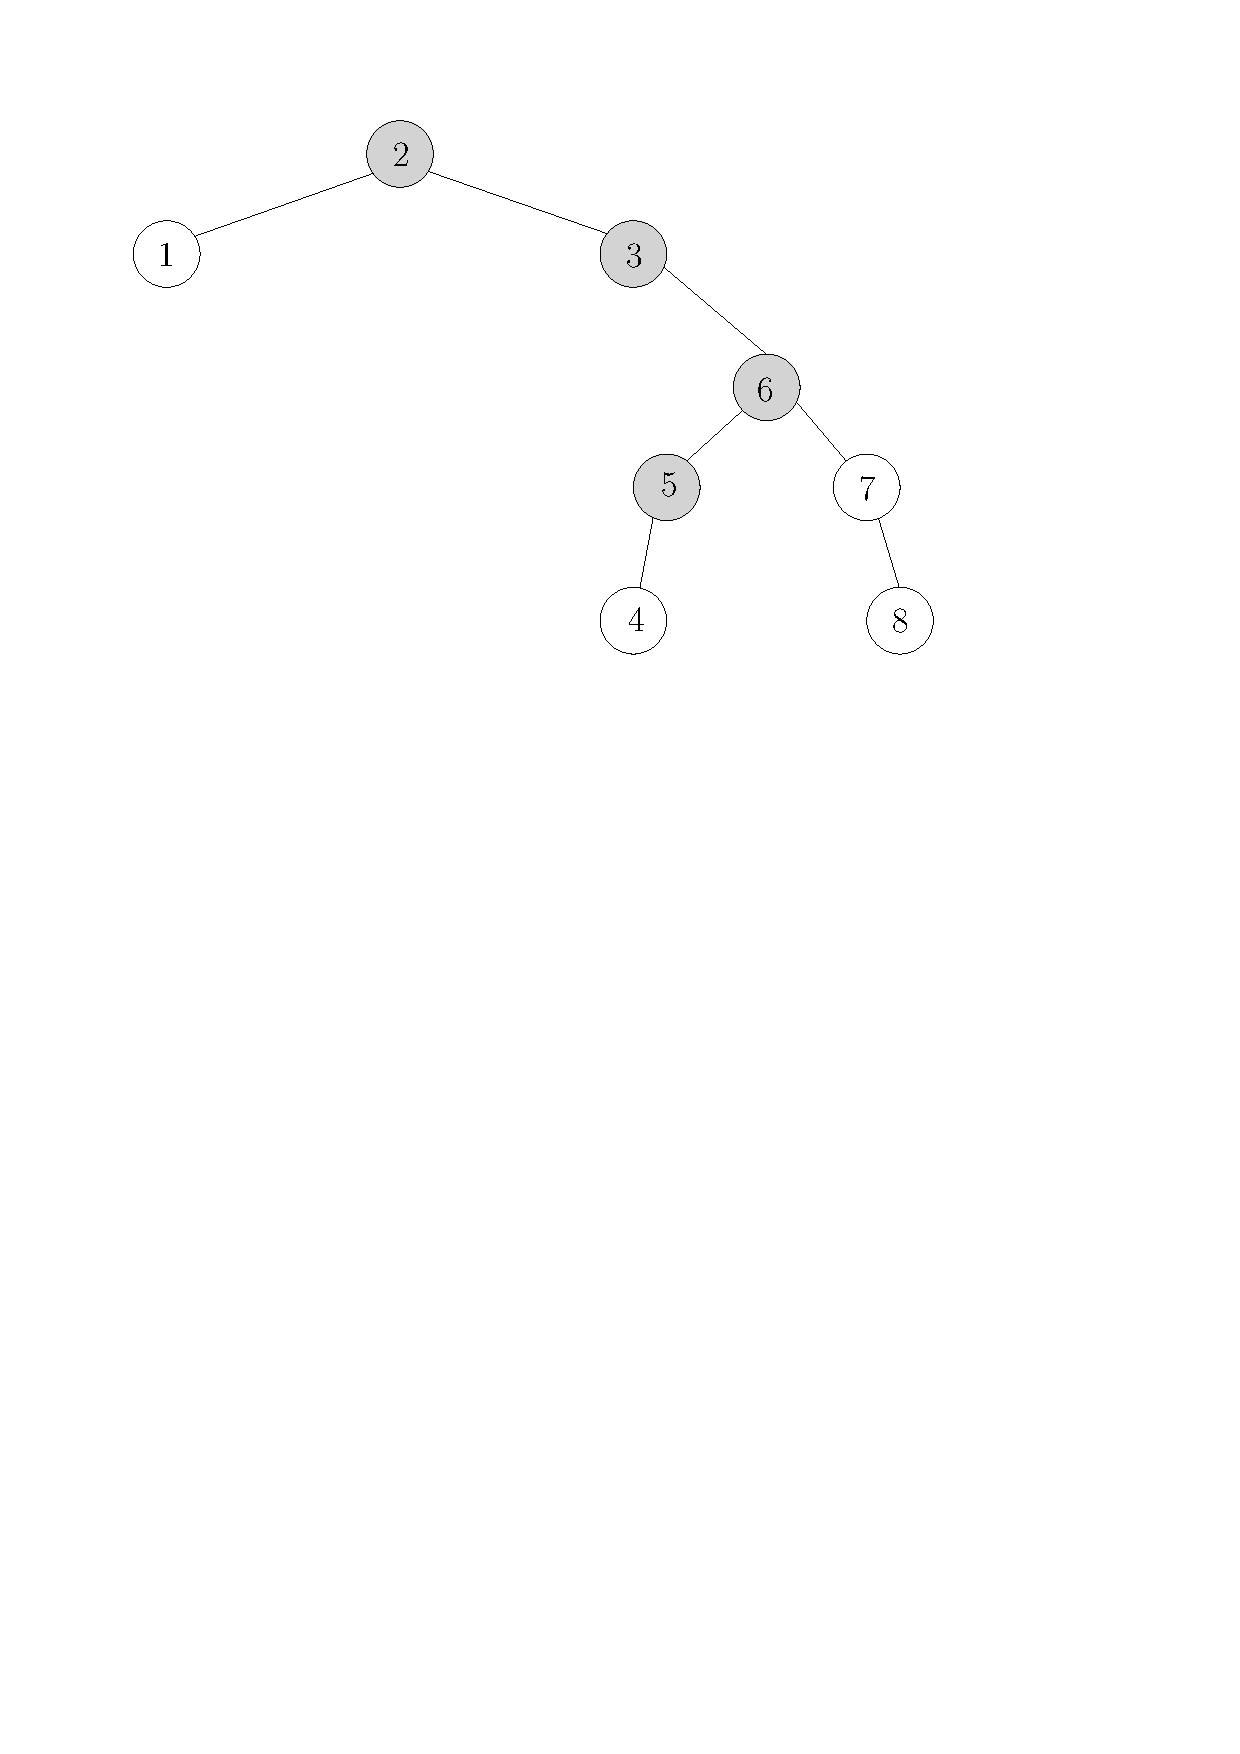
\includegraphics[width=0.6\textwidth]{qselect.pdf}
    \caption{quickselect for the $5^\text{th}$ largest element in $[2,3,6,1,7,5,8,4]$ with gray nodes visited}
\end{figure}

\newpage
\begin{thm}{}{}
    Let $B_{i,j,k}$ be an indicator variable which is 1 if $i$ is a common ancestor of  $j$ and $k$ in the quicksort tree. That is, if both $j$ and $k$ appear in the subtree $T(\pi)$ rooted at $i$.
    
    What is $\mathbb{E}[B_{i,j,k}]$? Give a succinct formula for this.
\end{thm}

\begin{proof}[Solution]
    Let's go down through the path that the algorithm visits.
    
    Suppose we are at the node whose pivot is $p$. If $p > \max\{i,j,k\}$ or $p < \min\{i,j,k\}$, then $i,j,k$ are all in the left subtree or all in the right subtree, which means we have to check one of the subtrees to determine $B_{i,j,k}$.
      
    If $\min\{i,j,k\} \leqslant p \leqslant \max\{i,j,k\}$, we can determine $B_{i,j,k}$ without going downwards, but we have to discuss some cases:
    \begin{enumerate}
        \item If $p=i$, then $B_{i,j,k}=1$ because $i$ is the ancestor of $j$ and $k$.
        \item If the condition of case 1 doesn't hold and $p\ne j$ and $p\ne k$, then $i,j,k$ are not in the same subtree. So $B_{i,j,k}=0$.
        \item If the condition of both case 1 and 2 don't hold, then either $j$ or $k$ is the ancestor of $i$. So $B_{i,j,k}=0$.
    \end{enumerate}
    
    In conclusion,  $B_{i,j,k}=1$ if and only if $i$ appears first among $[\min\{i,j,k\},\max\{i,j,k\}]$ in the input array. So  $\mathbb{E}[B_{i,j,k}]=\frac{1}{|[\min\{i,j,k\},\max\{i,j,k\}]|}=\frac{1}{\max\{i,j,k\}-\min\{i,j,k\}+1}$.
\end{proof}

\begin{thm}{}{}
    Let $C(\pi,k)$ be the number of comparisons made by \textsc{QuickSelect} when given $\pi$ as input. Design a formula for $C(\pi,k)$ with the help of the indicator variables $A_{i,j}$ and $B_{i,j,k}$ (analogous to the formula $\sum_{i\ne j}A_{i,j}$) for the number of comparisons made by quicksort).
\end{thm}

\begin{proof}[Solution]
    Observe that two numbers $i,j$ will be compared if and only if $j\ne i$ and $j$ and $k$ are in the subtree of $i$. An interpretation is that $i$ will be a pivot if and only if $i$ is on the path from root to node $k$, which is equal to $k$ is in the subtree rooted at $i$. As a pivot, $i$ will be compared to every node in the subtree rooted at $i$.
    
    So $C(\pi,k)=\sum_{i\ne j}B_{i,j,k}$.
\end{proof}

\newpage
\begin{thm}{}{}
    On expection, how many comparisions will it make to use QUICKSELECT to find the minimum of the array. 
\end{thm}
    Using the analysis in exercise 9(see below \ref{thm:t9}), we can get that 
    \begin{math}
        \sum_{1\leq i<j\leq n} B_{i,j,k}&= \sum_{i=1}^{k-1}\sum_{j=i+1}^{k} B_{i,j,k}+\sum_{i=k}^{n-1}\sum_{j=i+1}^{n} B_{i,j,k}\\
                                        &= k-H_k+n-(k+1)-H_{n-k+1}\\
                                        &= 1-H_1+n-2-H_n\\
                                        &= n - 2 - H_n\\
                                        &= n - \log(n) - 2 + o(1)
    .\end{math}

\begin{thm}{T9}{t9}
    Derive a formula for $\mathbb{E}_\pi[C(\pi, k)]$, up to additive terms of order $o(n)$. You might want to introduce $\kappa = k / n$.
\end{thm}

\begin{itemize}
    \item case $i<j\leq k$: 
        \begin{math}
            \sum_{i=1}^{k-1}\sum_{j=i+1}^{k} B_{i,j,k}&=\sum_{i=1}^{k-1}\frac{1}{k-i+1}*(k-i)\\
                                                      &=\sum_{i=1}^{k-1}(1-\frac{1}{k-i+1})=k-(1+\frac{1}{2}+\frac{1}{3}+\dots\frac{1}{k})\\
                                                      &= k - H_k
        .\end{math}
    \item case $k\leq i<j$:
        \begin{math}
            \sum_{i=k}^{n-1}\sum_{j=i+1}^{n} B_{i,j,k}&=\sum_{j=k+1}^{n}\sum_{i=k}^{j-1} B_{i,j,k}\\
                                                      &=\sum_{j=k+1}^{n}\frac{j-k}{j-k+1}\\
                                                      &=\sum_{j=k+1}^{n}(1-\frac{1}{j-k+1})\\
                                                      &=n-k+1-(1+\frac{1}{2}+\frac{1}{3}+\dots+\frac{1}{n-k+1})\\
                                                      &=n-k+1-H_{n-k+1}
        .\end{math}
\end{itemize}

\begin{itemize}
    \item case $i<k<j$:
        \begin{math}
            \sum _{i=1}^{k-1} \sum _{j=k+1}^n \frac{1}{j-i+1} &< \sum _{i=1}^{k-1} \int_{k+1}^{n+1} \frac{1}{j-i} \mathrm{d} j \\
                                              &= \sum _{i=1}^{k-1} \ln(n+1-i) - \ln(k+1-i) \\
                                              &< \int_{i=0}^{k-1} \ln(n+1-i) - \ln(k-i) \mathrm{d} i \\
                                              &= (n+1)\ln(n+1) - k\ln k - (n-k+2)\ln(n-k+2)
        .\end{math}

        On the other hand, similarly we can have
        \begin{math}
            \sum _{i=1}^{k-1} \sum _{j=k+1}^n \frac{1}{j-i+1} &> -(-k+n+2) \ln (-k+n+2)-(k+2) \ln (k+2)+(n+1) \ln (n+1)+3 \ln (3)
        .\end{math}

        The difference between the upper bound and the lower bound is $o(n)$, thus the inaccuracy is $o(n)$.

        To write this formula more simply, we have
        \begin{math}
            \sum _{i=1}^{k-1} \sum _{j=k+1}^n \frac{1}{j-i+1} = n \ln n - k \ln k - (n-k) \ln (n-k) + o(n)
        .\end{math}

        Summing three terms up, and multiply it by 2(because there are two possible orders between $i$ and $j$),
        \begin{math}
            \mathbb{E}_\pi[C(\pi,k)] &= 2(n + n\ln n - k\ln k - (n-k)\ln (n-k)) + o(n) \\
                                     &= 2(1+\ln \frac{1}{1-\kappa} + \kappa \ln \frac{1-\kappa}{\kappa})n + o(n)
        .\end{math}

\end{itemize}

\end{document}
